\documentclass{article}
\usepackage{polski}
\usepackage[utf8]{inputenc}
\usepackage{graphicx}
\usepackage{amsmath}
\usepackage{amssymb}
\usepackage{mathtools}

\title{Teoria Regulacji Ćwiczenia, Wtorek 17:05-18:45}
\author{Jan Bronicki 249011 }
\date{}

\begin{document}

\maketitle


\begin{center}
    Lista 3
\end{center}

\section*{Zadanie 1}

Niech $ M(s) = a_{m}s^{m}+a_{m-1}s^{m-1} + ... + a_{1}s+a_{0}$ to nasz wielomian charakterystyczny.
Niech $a_{m}>0$

\begin{itemize}

    \item[a)] $\frac{1}{s^{4}+7s^{3}+17s^{2}+17s+16}$
    Wszystkie współczynniki są dodatnie co oznacza, że system MOŻE być stabilny.
    Tworzymy macierz:

    $$ H=
    \begin{bmatrix}
        7 & 17 & 0 & 0\\
        1 & 17 & 6 & 0\\
        0 & 7 & 17 & 0\\
        0 & 1 & 17 & 6
        \end{bmatrix}$$

    Kryterium Hurwitza:

    \[\begin{cases}
        \Delta_{1}=7\\
        \Delta_{2}=102\\
        \Delta_{3}=1440\\
        \Delta_{4}=a_{0}\cdot \Delta_{3}=8640
    \end{cases}\]

    $$ \Delta_{1}, \Delta_{2}, \Delta_{3}, \Delta_{4}, > 0 $$
    
    Układ jest stabilny, brak pierwiastków w części rzeczywistej dodatniej oraz urojonej

    Kryterium Michajłowa:
    $$M(s)=s^{4}+7s^{3}+17s^{2}+17s+6$$
    $$ M(j\omega)=(\omega^{4}-17\omega^{2}+6)+(-7\omega^{3}+17\omega)j $$

    $$ Re(M(j\omega))=0 $$

    Niech $t=\omega^{2} $ i $ \omega^{2}>0$

    $$t^{2}-17t+6=0$$

    \[\begin{cases}
        t_{1}=\frac{17+\sqrt{265}}{2}
        \\
        t_{2}=\frac{17-\sqrt{265}}{2}
    \end{cases}\]

    \[\begin{cases}
        \omega_{1}=\sqrt{\frac{17+\sqrt{265}}{2}}
        \\
        \omega_{2}=-\sqrt{\frac{17+\sqrt{265}}{2}}
        \\
        \omega_{3}=\sqrt{\frac{17-\sqrt{265}}{2}}
        \\
        \omega_{4}=-\sqrt{\frac{17-\sqrt{265}}{2}}
    \end{cases}\]

    $$Im(M(j\omega))=0$$

    $$ -7\omega^{3}+17\omega=0 $$

    \[\begin{cases}
        \omega_{5}=0\\
        \omega_{6}=\sqrt{\frac{17}{7}}\\
        \omega_{7}=-\sqrt{\frac{17}{7}}
    \end{cases}\]

    Bierzemy pod uwagę tylko $\omega>=0$

    \[\begin{cases}
        \omega_{1}=4.1\\
        \omega_{3}=0.6\\
        \omega_{5}=0\\
        \omega_{6}=1.56
    \end{cases}\]

    $$\Delta argM(j\omega)_{0\leq \omega \le \infty }=m\frac{\pi}{2}=2\pi$$

    \begin{figure}[h!]
        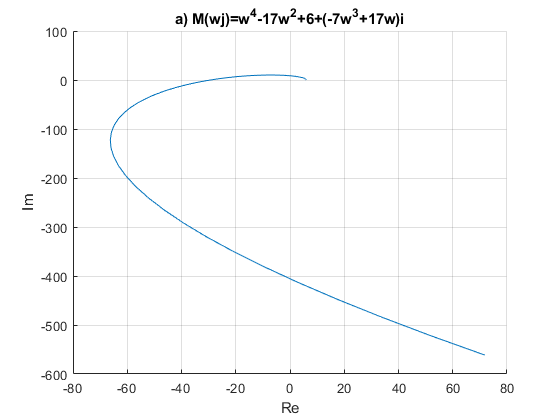
\includegraphics[scale=0.5]{a.png}
        \centering
    \end{figure}

    \newpage

    \item[b)] $\frac{s-2}{s^{4}+6s^{3}+13s^{2}+12s+4}$
    Może być stabilny.
    $$ H=
    \begin{bmatrix}
        6 & 12 &  0 & 0\\
        1 & 13 &  4 & 0\\
        0 &  6 & 12 & 0\\
        0 &  1 & 13 & 4
        \end{bmatrix}$$

    \[\begin{cases}
        \Delta_{1}=6\\
        \Delta_{2}=76\\
        \Delta_{3}=4\cdot144+6\cdot12\\
        \Delta_{4}=a_{0}\cdot \Delta_{3}=4(4\cdot12^{2}+6\cdot12)
    \end{cases}\]

    Kryterium Hurtwitza:

    $$ \Delta_{1}, \Delta_{2}, \Delta_{3}, \Delta_{4}, > 0 $$

    Układ stabilny, brak pierwiastków w części rzeczywistej dodatniej oraz urojonej

    Kryterium Michajłowa:
    
    $$M(s)=s^{4}+6s^{3}+13s^{2}+12s+4$$

    $$M(j\omega) = (\omega^{4}-13\omega^{2}+4) + (-6\omega^{3}+12\omega)j$$

    

    $$ Re(M(j\omega))=0 $$

    Niech $t=\omega^{2} $ i $ \omega^{2}>0$

    $$t^{2}-17t+6=0$$

    \[\begin{cases}
        t_{1}=\frac{17+\sqrt{265}}{2}
        \\
        t_{2}=\frac{17-\sqrt{265}}{2}
    \end{cases}\]

    \[\begin{cases}
        \omega_{1}=\sqrt{\frac{17+\sqrt{265}}{2}}
        \\
        \omega_{2}=-\sqrt{\frac{17+\sqrt{265}}{2}}
        \\
        \omega_{3}=\sqrt{\frac{17-\sqrt{265}}{2}}
        \\
        \omega_{4}=-\sqrt{\frac{17-\sqrt{265}}{2}}
    \end{cases}\]

    $$Im(M(j\omega))=0$$

    $$ -7\omega^{3}+17\omega=0 $$

    \[\begin{cases}
        \omega_{5}=0\\
        \omega_{6}=\sqrt{\frac{17}{7}}\\
        \omega_{7}=-\sqrt{\frac{17}{7}}
    \end{cases}\]

    Bierzemy pod uwagę tylko $\omega>=0$

    \[\begin{cases}
        \omega_{1}=4.1\\
        \omega_{3}=0.6\\
        \omega_{5}=0\\
        \omega_{6}=1.56
    \end{cases}\]

    $$\Delta argM(j\omega)_{0\leq \omega \le \infty }=m\frac{\pi}{2}=2\pi$$

    \begin{figure}[h!]
        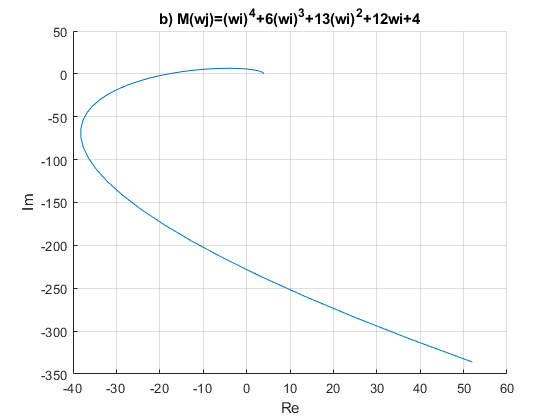
\includegraphics[scale=0.5]{b.png}
        \centering
    \end{figure}
    \newpage

    \item[c)] $\frac{s+3}{s^{3}+4s^{2}+s-6}$
    
    $$ a_{0}=-6<0 \ \text{niestabilny}$$

    $$ H=
    \begin{bmatrix}
        4 & -6 & 0\\
        1 & 1 &  0\\
        0 & 4 & -6\\
        \end{bmatrix}$$

    \[\begin{cases}
        \Delta_{0}=4\\
        \Delta_{1}=10\\
        \Delta_{2}=a_{0}\cdot \Delta_{1}=-60\\
    \end{cases}\]

    $$ V\left(4, \ \frac{10}{4}, -\frac{60}{10}\right)=1$$

    $$\Delta_{0}, \Delta_{1}, \Delta_{2}\neq 0$$

    $$ V\neq 0$$
    Niestabilny

    Michajłowa

    $$  M(\omega j ) = (\omega j)^{3}+4(\omega j)^{2}+\omega j - 6$$

    \begin{figure}[h!]
        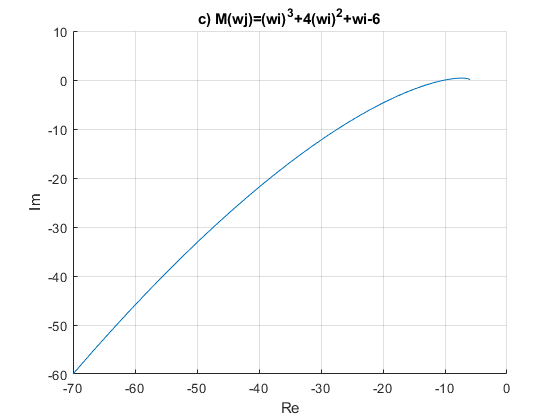
\includegraphics[scale=0.5]{c.png}
        \centering
    \end{figure}
    \newpage
    \item[d)] $\frac{s+4}{s^{3}+6s^{2}+11s+6}$

    Może być stabilny ponieważ współczynniki są dodatnie.

    
    $$ H=
    \begin{bmatrix}
        6 & 6  & 0\\
        1 & 11 & 0\\
        0 & 6  & 6\\
        \end{bmatrix}$$

    \[\begin{cases}
        \Delta_{0}=6\\
        \Delta_{1}=60\\
        \Delta_{2}=a_{0}\cdot \Delta_{1}=360\\
    \end{cases}\]



    $$ V\left(6, \ \frac{60}{6}, \frac{360}{60}\right)=0$$


    $$\Delta_{0}, \Delta_{1}, \Delta_{2}> 0$$ 
    Stabilne

    Michajłowa

    $$M(\omega j)=(\omega j)^{2}+6(\omega j )^{2}+11(\omega j)+6$$

    \begin{figure}
        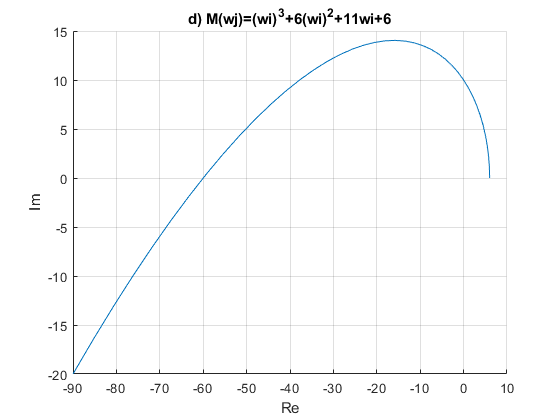
\includegraphics[scale=0.5]{d.png}
        \centering
    \end{figure}

\end{itemize}

\newpage

\section*{Zadanie 2}

$$s^{2}+a_{1}s+a_{0}=0$$
$$a_{1}, a_{0} > 0$$

$$ H_{2x2}=
    \begin{bmatrix}
        a_{1}& 0\\
        1& a_{0}\\
    \end{bmatrix}$$

    \[\begin{cases}
        \Delta_{1}=a_{1} > 0\\
        \Delta_{2}=a_{1}a_{0} > 0
    \end{cases}\]

    Z Hurwitza system jest stabilny zakładając, że $a_{1}>0$ oraz $a_{0}>0$.


\end{document}
